\section{数据、尺度与研究问题}
\subsection{三种分配模型为何分开评价}
基础课件关注双边在线问题：司机和请求逐步到达，平台只看已发生事件，每个司机只用一次。静态多目标问题则把一个批次的全部司机和OD一次给出，允许主动不派，研究接驾与收入的前沿。强化学习问题允许同一辆车完成一次出行后继续接单，派单还会改变未来车辆位置。三者的信息、容量和时间语义不同，因此不能把静态NSGA的效用比直接当作在线延迟竞争比，也不能用一次批次的收入替代全天模拟收入。

\begin{table}[htbp]\centering\caption{保持独立身份的主要教学场景。}\label{tab:scales}
\begin{tabularx}{\linewidth}{lYYY}\toprule
场景&对象与时间&空间与速度&成本/目标\\\midrule
基础课件&20司机、20请求，0--20 min&10×10 km，1 km/min&等待+欧氏接驾时间\\
基础Notebook&100司机、100请求，0--2000时间单位&0--1000空间单位，速度1单位/单位&抽象单位的延迟\\
静态进阶&40司机、80代理订单&曼哈顿3 km候选半径，每单最多6司机&车费代理、接驾km、服务数\\
动态车队&40/60/100车，6:00--24:00&8×8网格，25 km/h，10 min/片&接单收入、应答、接驾和调度成本\\\bottomrule
\end{tabularx}
\end{table}

\subsection{Foursquare签到怎样成为代理订单}
两份教师压缩包及其嵌套归档含相同城市数据，逐字节哈希证实重复副本相同，不把它们累计成更多样本。Foursquare数据追溯至原作者发布页\cite{foursquare}。实收NYC有227,428条签到，TKY有573,703条；本次仿真按教师NYC矩形与模型展开，TKY用于完整来源、字段和质量审计，没有未经确认另建东京运营场景。数据包含用户、场所、类别、经纬度、UTC时间与逐条时区偏移。签到不是出租车订单，两个相邻签到也不提供实际道路或行程。

按教师代码，先取纬度$[40.60,40.88]$、经度$[-74.05,-73.75]$内签到，再按用户和当地civil-clock排序。同一当地日期内，相邻保留签到间隔10--180 min、曼哈顿工作距离至少1 km时形成一个OD代理，得到25,550条。先做矩形筛选再相邻配对可能跨过矩形外的记录，这是代理机制的局限。

工作坐标为$x=(\mathrm{lon}+74.05)\,111\cos40.74^\circ$、$y=(\mathrm{lat}-40.60)\,111$，以教学近似km计算。文件没有独立的datum证明，因此不将该模型解释为已确认的绝对地理精度。进阶车费代理为$5+2d_{OD}$，基础NSGA只用欧氏送客距离表示收入，二者不混用。

\subsection{时间审计与训练、选择、确认}
每条UTC加该记录的分钟偏移形成当地时间。独立取回OD两端的原始来源行后发现，12对的UTC实际间隔与当地钟面差不一致，其中6对UTC倒序，且12对都不满足UTC的10--180 min窗口。因此主基线准确称为教师local-clock代理，不能据此断言真实出行时长。保留原始值，另以剔除这12对的副本做训练内稳健性，不静默更换数据定义。

按代理记录的不同日期排序，前70\%日期为训练大区间、后30\%保持测试；训练大区间的后20\%日期用作验证，前段为inner训练。对应inner有19,617条/139个日期，验证1,972条/35个日期，测试3,961条/75个日期；分界分别为2012年10月19日与11月27日。模拟日从相应池中重采样1500单，训练300回合是300次仿真，不能写成300个真实运营日。

原Notebook从全量签到采样司机热点，会让未来测试位置进入训练条件。本次将开发的初始司机严格限制到inner签到，最终重训后只用前70\%签到。验证用于选择，测试只作冻结后的确认；用于全量描述的统计不当作训练特征。两城市原始数据中的重复、起止日期与作者网页/README差异均保留审计，不根据课件参考条数修改源文件。

\begin{figure}[htbp]\centering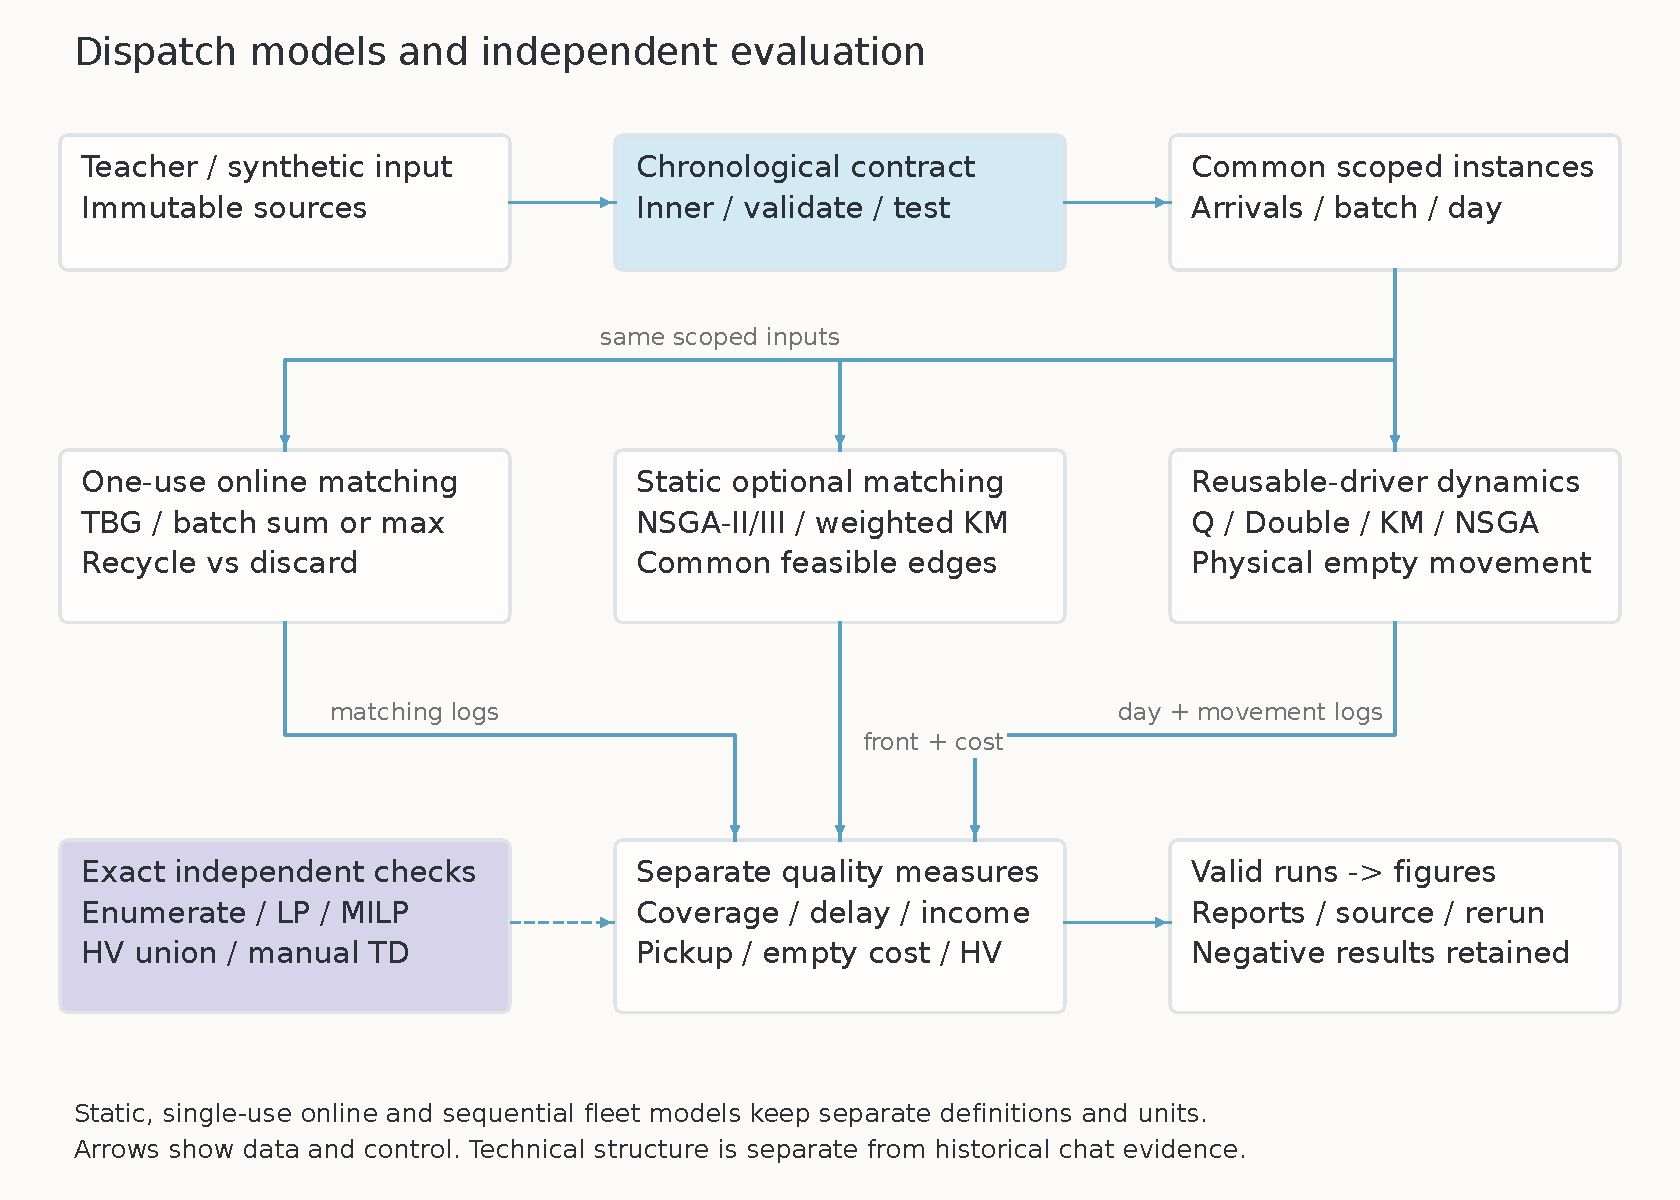
\includegraphics[width=\linewidth]{../../diagrams/dispatch_runtime_and_evaluation.pdf}
\caption{本次实现的三个模型与共同核验关系。静态、单次在线和跨时间车队采用不同容量语义，参考求解器与结果指标分开。图中箭头表示实际技术依赖。}\label{fig:runtime}\end{figure}
